\documentclass{standalone}
\usepackage{tikz}
\usetikzlibrary[arrows,positioning,matrix]

\begin{document}
\begin{tikzpicture}
  \node[draw=none] (randomcontrol) {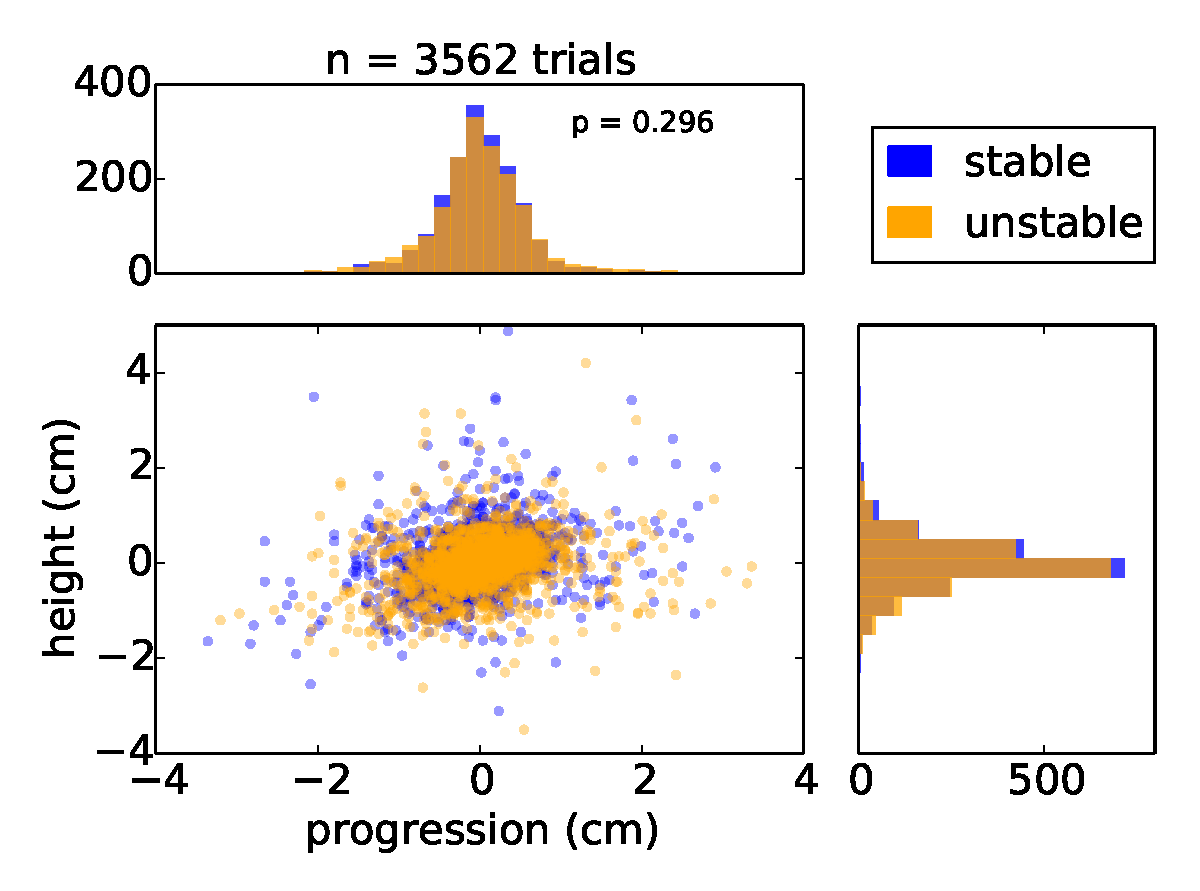
\includegraphics[width=0.5\textwidth]{elements/randomcontrol}};
  \node[draw=none,above=-2mm of randomcontrol] {current state};
  \node[draw=none,above left=-5mm and -5mm of randomcontrol] {A};

  \node[draw=none,right=1mm of randomcontrol] (randombias) {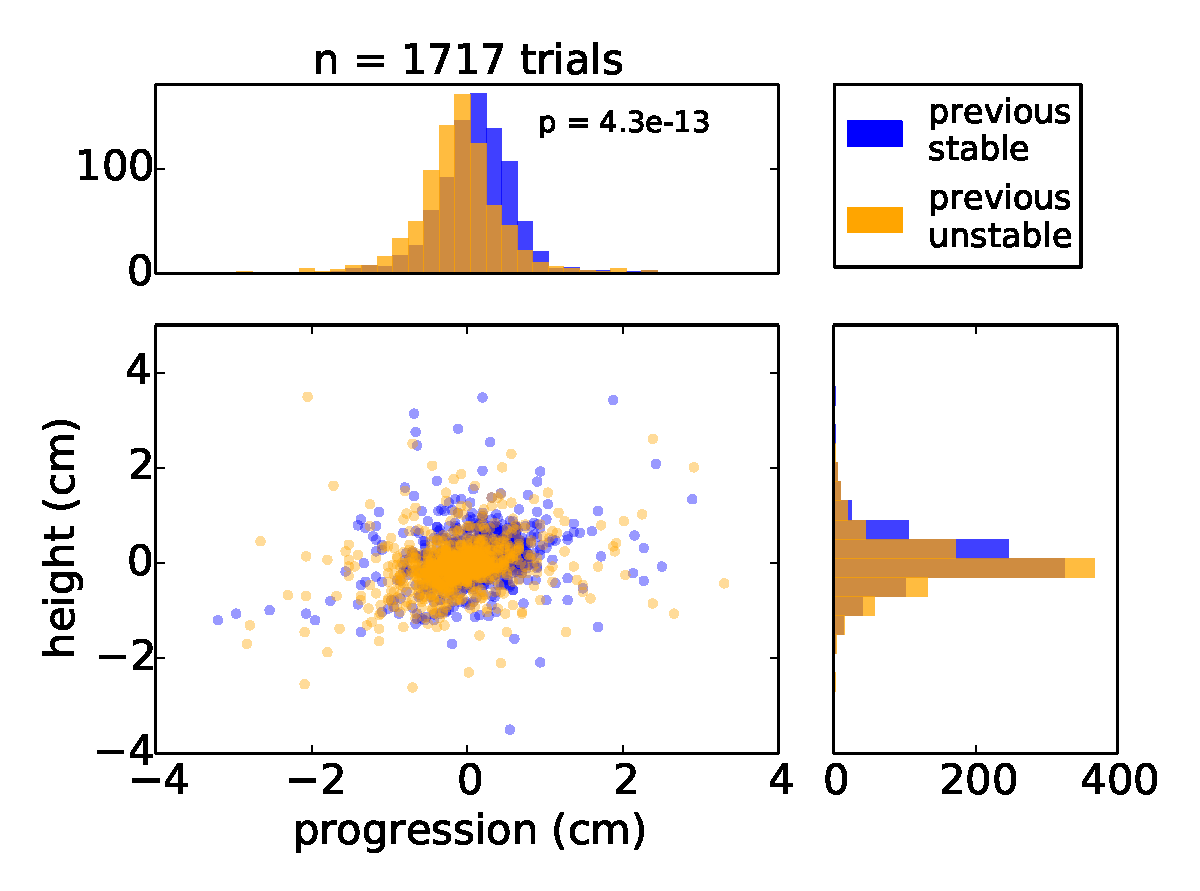
\includegraphics[width=0.5\textwidth]{elements/randombias}};
  \node[draw=none,above=-2mm of randombias] {previous state};
  \node[draw=none,above left=-5mm and -5mm of randombias] {B};
  
  \node[draw=none,below=0.5cm of randomcontrol] (randombiascontrols) {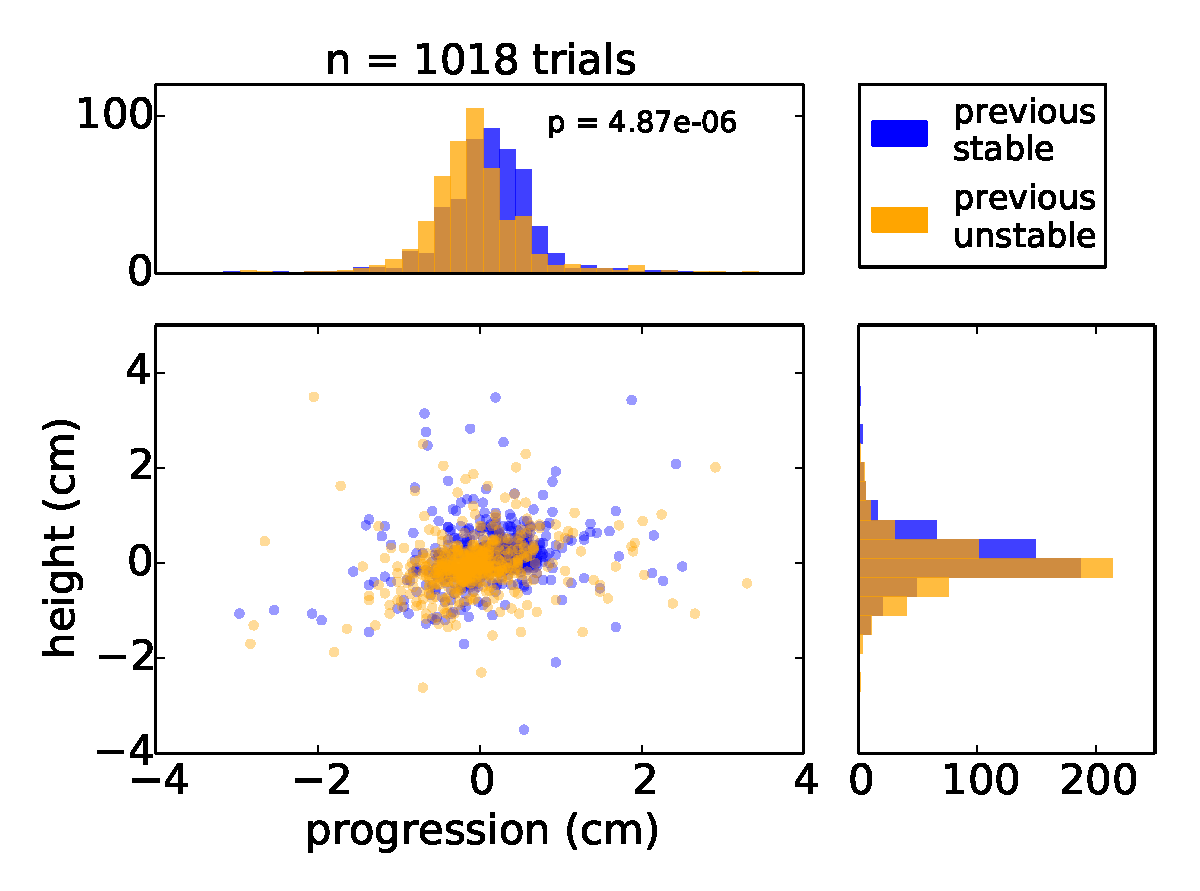
\includegraphics[width=0.5\textwidth]{elements/randombias_controls}};
  \node[draw=none,above=-2mm of randombiascontrols] {controls};
  \node[draw=none,above left=-5mm and -5mm of randombiascontrols] {C};
  
  \node[draw=none,right=1mm of randombiascontrols] (randombiaslesions) {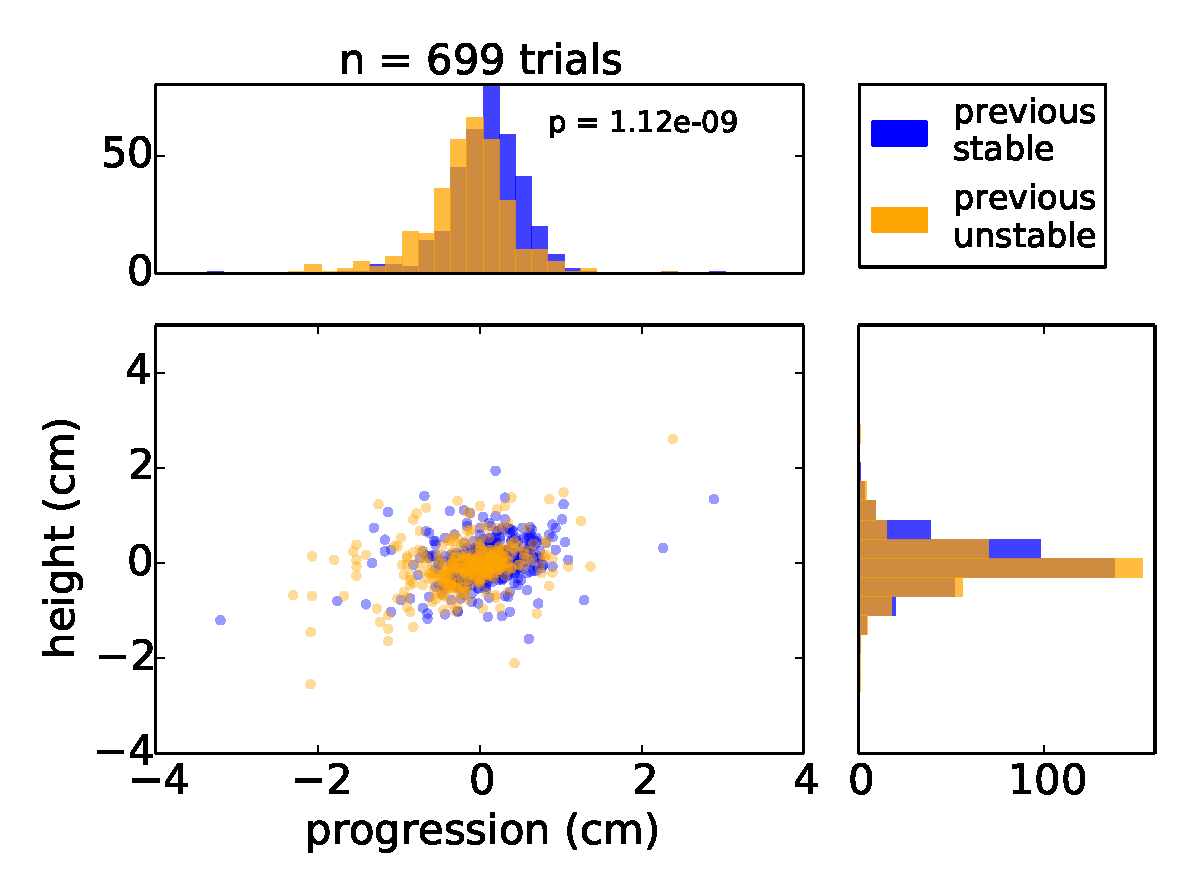
\includegraphics[width=0.5\textwidth]{elements/randombias_alllesions}};
  \node[draw=none,above=-2mm of randombiaslesions] {lesions};
  \node[draw=none,above left=-5mm and -5mm of randombiaslesions] {D};
\end{tikzpicture}
\end{document}